\documentclass[a4paper]{article}
\usepackage{booktabs}
\usepackage{geometry}
\geometry{
  top=1in,
  inner=1in,
  outer=1in,
  bottom=1in,
  headheight=3ex,
  headsep=2ex
}
\usepackage{amssymb,amsmath}
\usepackage{fontspec}
\usepackage[CJKbookmarks, colorlinks, bookmarksnumbered=true,pdfstartview=FitH,linkcolor=black,citecolor=black]{hyperref}
\usepackage{xeCJK}
\usepackage{xltxtra,xunicode}
\usepackage{listings}
\usepackage{xcolor}
\usepackage{array}

\lstset{basicstyle=\footnotesize\ttfamily,        % size of fonts used for the code
        columns=fullflexible,
        numbers=left,
        numberstyle=\tiny,
        keywordstyle=\color{blue},
        stringstyle=\color[rgb]{0,0.6,0},
        commentstyle=\color[cmyk]{1,0,1,0},
        frame=shadowbox,
        escapeinside=``,
        breaklines=true,
        extendedchars=false,
        xleftmargin=2em,xrightmargin=2em, aboveskip=1em,
        tabsize=4, %tab size
        showspaces=false %no space
       }

\newcommand{\tightlist}{
  \setlength{\itemsep}{0pt}\setlength{\parskip}{0pt}}

% font
\setCJKmainfont[AutoFakeBold]{文泉驿微米黑}
\setmainfont[AutoFakeBold]{Segoe UI}
\setromanfont[AutoFakeBold]{Segoe UI}
\setmonofont[Mapping={}]{Monaco}
\linespread{1.2}\selectfont
\XeTeXlinebreaklocale "zh" 

\begin{document}
\title{\Huge 算法导论课程\\ 第四次上机实验报告}
\author { \vspace{12cm} \\ \LARGE 班级:  1413014  \\ \LARGE 姓名:  乔新文   \\ \LARGE 学号:14130140393} 
\date{ \vspace{4cm} 2017.5.8}

\maketitle
\clearpage

\tableofcontents

\clearpage

\section{综述}

本文档将阐述《算法导论》第四次上机实验代码的详细设计及实现。\\

本次上机实验所用代码均为F\#代码,主要算法和辅助定义均包含在SRAlgorithmLib命名空间下AlgorithmLib4.fs所定义的AlgorithmLib4模块中。\\

算法测试驱动部分在Test.fs中Test模块下的P4函数中,整个程序的入口在Program.fs中。\\

本次实验所有代码均运行在.Net Core上,P1.fsproj为项目配置文件,可在安装有.Net Core的环境中在项目文件夹下使用dotnet run命令运行。\\

\section{题目一}

\subsection{题目}

Bellman-Ford algorithm 

\subsection{实现思路}
Bellman-Ford算法通过对边进行松弛来渐进的降低从源节点到每个节点的最短路径的估计值,并侦测是否存在可以从源节点到达的权重为负值的环路。
\subsection{实现代码}

节点的类型定义\\
其中name记录节点的编号,d记录从源节点到此节点的最短路径权重的上界,π记录其前驱节点
\begin{lstlisting}[language=ML]
    [<Class>]
    type Vertex = 
        val name : int
        val mutable d : float
        val mutable π : Vertex ref option
        new (_name : int, D : float, PI : Vertex ref option) = {name=_name; d=D; π=PI}
\end{lstlisting}

边的类型定义\\
其中u,v记录了边的起始节点和终止节点,weight记录从了边的权重
\begin{lstlisting}[language=ML]
    [<Class>]
    type Edge = 
        val u : Vertex ref
        val v : Vertex ref
        val weight : float
        new (U : Vertex ref, V : Vertex ref, _weight : float) = {u=U; v=V; weight=_weight}
\end{lstlisting}

图的类型定义\\
其中包含边的集合和节点的集合,由邻接矩阵创建并初始化每个节点的d和π
\begin{lstlisting}[language=ML]
    [<Class>]
    type Graphics (adjMatrix : float [,]) as this =
        do
            this.V <- [for i in 0..(Array2D.length1 adjMatrix - 1) -> Vertex(i,infinity,None)]
            this.E <- [
                for i in 0..(Array2D.length1 adjMatrix - 1) do
                    for j in 0..(Array2D.length2 adjMatrix - 1) do
                        if adjMatrix.[i,j] <> infinity || adjMatrix.[i,j] <> 0.0 then
                            yield Edge(ref this.V.[i], ref this.V.[j], adjMatrix.[i,j])
            ]
        [<DefaultValue>] val mutable V : Vertex List
        [<DefaultValue>] val mutable E : Edge List
\end{lstlisting}

初始化操作\\
由于新建图时每个顶点的d和π已被初始化,故这里只设置源节点的d
\begin{lstlisting}[language=ML]
    let InitializeSingleSource (G:Graphics) (s:int) =
        G.V.[s].d <- 0.0
\end{lstlisting}

松弛操作
\begin{lstlisting}[language=ML]
    let Relax (e:Edge)= 
        if (!e.v).d > (!e.u).d + e.weight then
            (!e.v).d <- (!e.u).d + e.weight
            (!e.v).π <- Some(e.v)
\end{lstlisting}

Bellman-Ford算法
\begin{lstlisting}[language=ML]
    let BellmanFord (G:float [,]) (s:int)= 
        let g = Graphics(G)
        InitializeSingleSource g s
        for i = 0 to g.V.Length - 2 do
            List.iter Relax g.E
        not (
                List.exists (fun (item : Edge) -> 
                    (!item.v).d > (!item.u).d + item.weight
                ) g.E
            )
\end{lstlisting}

\subsection{算法测试}

\begin{itemize}
\item
    测试样例:
    \begin{itemize}
    \item
        设置起点为0(无负权回路)\\
       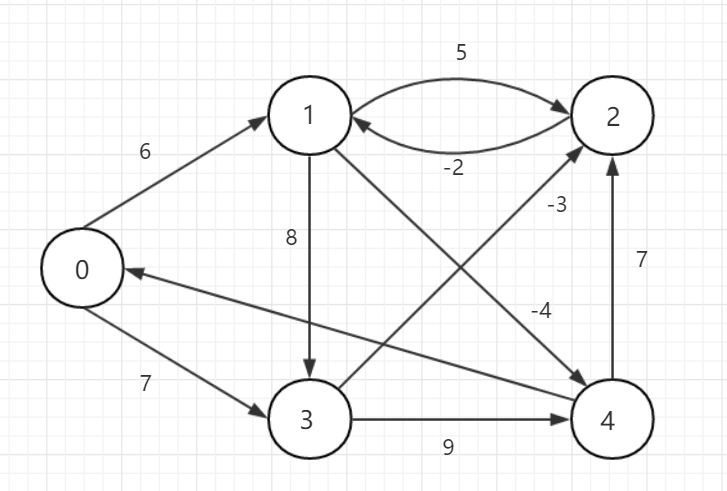
\includegraphics[width=8cm]{4-1-1.png}
    \item
        设置起点为0(存在负权回路)\\
       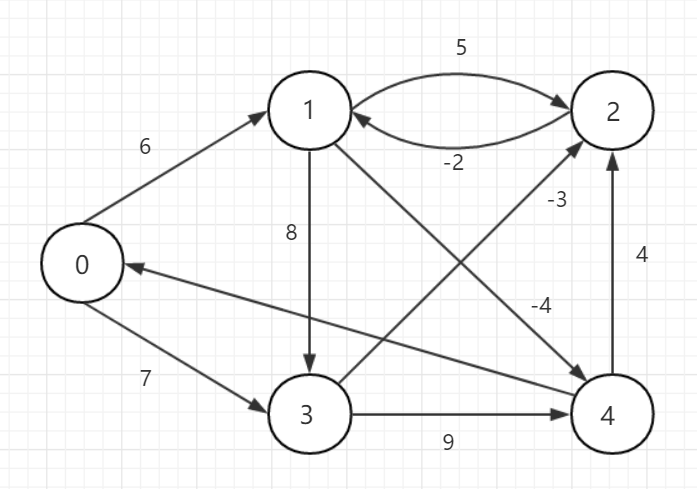
\includegraphics[width=8cm]{4-1-2.png}
    \end{itemize}
\item
    样例输出
    \begin{itemize}
    \item
        true
    \item
        false
    \end{itemize}
\end{itemize}


\section{题目二}

\subsection{题目}

All-pairs shortest path (choose one from the three algorithms)

\subsection{实现思路}

使用动态规划的Floyd算法求解。\\
最短路径的递归求解公式为:
\[c[i,j,k]=
    \left\{
        \begin{array}{ll}
            0 & ,i=j\\
            g[i,j] & ,k=0\\
            min(c[i,j,k-1],c[i,k,k-1]+c[k,j,k-1]) & ,k>0
        \end{array}
    \right.
\]
\subsection{实现代码}

定义邻接链表的节点元素。

\begin{lstlisting}[language=ML]
    [<Struct>]
    type Node = 
            val ID:int
            val Weight:float
            new (id:int,weight:float) = {ID = id; Weight = weight}
\end{lstlisting}

邻接链表到邻接矩阵的转换方法

\begin{lstlisting}[language=ML]
    let AdjListToAdjMatrix (adjList : Set<Node>[]) =
        let adjMatrix = Array2D.create adjList.Length adjList.Length infinity
        for i = 0 to adjList.Length - 1 do
            adjMatrix.[i,i] <- 0.0
            for j in adjList.[i] do
                adjMatrix.[i,j.ID] <- j.Weight
        
        adjMatrix
\end{lstlisting}

计算所有节点对间最短距离的Floyd算法\\
其中,m保存了节点间的最短距离,s保存了节点对间最短路径上的中间节点

\begin{lstlisting}[language=ML]
    let Floyd (G:float [,]) = 
        let n = Array2D.length1 G
        let m = Array2D.copy G
        let s = Array2D.create n n -1
        for i = 0 to n - 1 do
            for j = 0 to n - 1 do
                for k = 1 to n - 1 do
                    let q = m.[i,k] + m.[k,j]
                    if q < m.[i,j] then
                         m.[i,j] <- q
                         s.[i,j] <- k
        (m,s)
\end{lstlisting}

递归的打印最短路径

\begin{lstlisting}[language=ML]
    let rec PrintFloyd (s:int [,]) (i:int) (j:int) = 
        if i = j then
            printf "%A " i
        elif s.[i,j] = -1 then
            printf "%A %A " i j
        else
            PrintFloyd s i s.[i,j]
            PrintFloyd s s.[i,j] j
\end{lstlisting}

\subsection{算法测试}

\begin{itemize}
\item
    测试样例:
    \begin{itemize}
    \item
        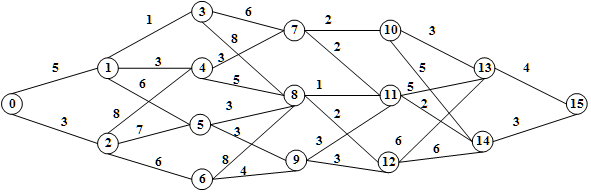
\includegraphics[width=12cm]{4-2.png}
    \end{itemize}
\item
    样例输出
    \begin{itemize}
    \item
        0 1 1 4 4 7 7 11 11 14 14 15
    \end{itemize}
\end{itemize}

\section{题目三}

\subsection{题目}

8-queen problem (back backing)

\subsection{实现思路}

使用具有贪心性质的最短作业优先调度方案。\\
对于有任意数目的作业的情况,\(j_1\)在\(t_1\)时间结束,\(j_2\)在\(t_1+t_2\)时间结束,以此类推,平均周转时间为 \[(n*t_1+(n-1)*t_2+(n-2)*t3+...+2*t_{n-1}+t_n) \div n\]
可见\(t_1\)对平均周转时间的影响最大,\(t_2\)次之,\(t_n\)最小,故应使\(j_1\)为最短作业,\(j_n\)为最长作业。
\subsection{实现代码}

按照短作业优先策略计算平均周转时间

\begin{lstlisting}[language=ML]
    let SJF j t =
        let jobsAndTime = List.zip j t
        let jobsSortedByTime = List.sortBy (fun item -> item |> snd) jobsAndTime
        let (j',t') = List.unzip jobsSortedByTime
        let sumTime = List.mapi (fun i item -> float (item * (t'.Length - i))) t'
        (j',List.average sumTime)
\end{lstlisting}

其中:\\

\begin{lstlisting}[language=ML]
        let jobsAndTime = List.zip j t
        let jobsSortedByTime = List.sortBy (fun item -> item |> snd) jobsAndTime
        let (j',t') = List.unzip jobsSortedByTime
\end{lstlisting}
用于对作业持续时间进行升序排列,并保持与任务名称列表间的对应关系。

\begin{lstlisting}[language=ML]
        let sumTime = List.mapi (fun i item -> float (item * (t'.Length - i))) t'
        (j',List.average sumTime)
\end{lstlisting}

用于计算平均周转时间并返回计算结果和作业调度序列。

\subsection{算法测试}

\begin{itemize}
\item
    测试样例:
    \begin{itemize}
    \item
        作业序列 \ [j1;j2;j3;j4] \\
        作业持续时间 \ [15;8;3;10]
    \end{itemize}
\item
    样例输出
    \begin{itemize}
    \item
        平均周转时间最短的作业安排 \ [j3; j2; j4; j1] \\
        最短的平均周转时间 \ 17.75
    \end{itemize}
\end{itemize}

\section{题目四}

\subsection{题目}

Bin Packing

\subsection{实现思路}

使用贪心策略,从最大的物品开始装起,并尽可能将箱子装满。

\subsection{实现代码}

判断当前是否还有箱子可以装下次物品,若有,返回该箱子的索引。若没有,返回Null。\\
由于浮点数计算存在精度问题,故限定可接受的误差在0.000001内。

\begin{lstlisting}[language=ML]
            let index = Array.tryFindIndex (fun box -> (box - item) > -0.000001) boxs
\end{lstlisting}

若箱子可以装下,则装入该箱子并更新箱子剩余容量。\\
若装不下,则新放入一个箱子并装入。

\begin{lstlisting}[language=ML]
            if index.IsSome then
                boxs.[index.Value] <- boxs.[index.Value] - item
            else
                boxs <- Array.append boxs [|1.0 - item|]
\end{lstlisting}

对箱子按照剩余容量降序排序,因为物品是按降序装入的,可以让剩余容量大的箱子尽可能装满。

\begin{lstlisting}[language=ML]
            boxs <- Array.rev (Array.sort boxs)
\end{lstlisting}

完整的Packing代码如下:

\begin{lstlisting}[language=ML]
    let Packing c s =
        let s' = List.rev (List.sort s)
        let mutable boxs = Array.create 0 1.0
        List.iter (fun item -> 
            let index = Array.tryFindIndex (fun box -> (box - item) >= -0.000001 ) boxs
            if index.IsSome then
                boxs.[index.Value] <- boxs.[index.Value] - item
            else
                boxs <- Array.append boxs [|1.0 - item|]
            boxs <- Array.rev (Array.sort boxs)
            ) s'
        boxs.Length
\end{lstlisting}

\subsection{算法测试}

\begin{itemize}
\item
    测试样例:
    \begin{itemize}
    \item
        物品尺寸序列 \ [ 0.5;0.7;0.3;0.9;0.6;0.8;0.1;0.4;0.2;0.5] 
    \end{itemize}
\item
    样例输出
    \begin{itemize}
    \item
        需要的箱子数 \ 5
    \end{itemize}
\end{itemize}

\end{document}